\documentclass[]{article}
\usepackage{graphicx}

%opening
\title{Tables}
\author{Mao Hu}

\begin{document}

\maketitle

\textbf{Comment on simulations}
Simulations were conducted using Lynn's priors, with unspecified priors (i.e. those not in the prior table, not in either of the US or Canada datasets) being set to $0.5$.  Only 45 simulations of each of the 9 models were run due to time constraints.  Additional code was used to ``patch" a possible bug in the \texttt{bic.glm.data.frame} function within the \texttt{BMA} package, although I haven't confirmed that this is true bug.

\begin{figure}[h]
\caption{Coefficients in True Models Used in Simulation}
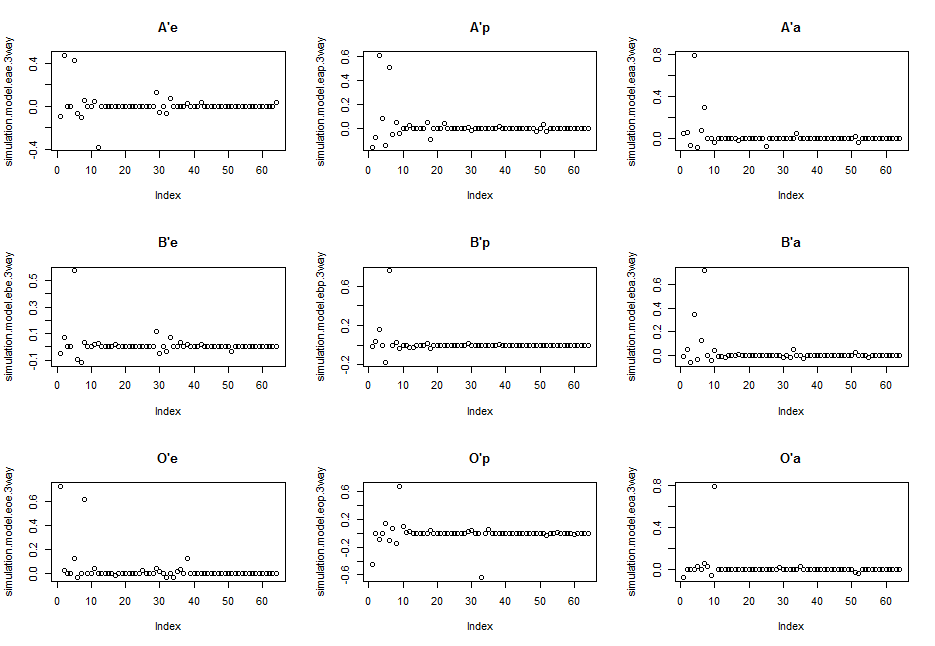
\includegraphics[width=15cm]{Rplot.png}
\caption{The x-axis consists of Intercept, 9 main effects, 27 second order interactions, and 27 third order interaction terms, in that order.  Coefficients which are nonzero are in the true model. Observe that evaluation models look "more complicated" than the activity models. }
\end{figure}
\begin{verbatim}
[1] "(Intercept)" "ae"          "ap"          "aa"          "be"         
 [6] "bp"          "ba"          "oe"          "op"          "oa"         
[11] "ae.be"       "ae.bp"       "ae.ba"       "ae.oe"       "ae.op"      
[16] "ae.oa"       "ap.be"       "ap.bp"       "ap.ba"       "ap.oe"      
[21] "ap.op"       "ap.oa"       "aa.be"       "aa.bp"       "aa.ba"      
[26] "aa.oe"       "aa.op"       "aa.oa"       "be.oe"       "be.op"      
[31] "be.oa"       "bp.oe"       "bp.op"       "bp.oa"       "ba.oe"      
[36] "ba.op"       "ba.oa"       "ae.be.oe"    "ae.be.op"    "ae.be.oa"   
[41] "ae.bp.oe"    "ae.bp.op"    "ae.bp.oa"    "ae.ba.oe"    "ae.ba.op"   
[46] "ae.ba.oa"    "ap.be.oe"    "ap.be.op"    "ap.be.oa"    "ap.bp.oe"   
[51] "ap.bp.op"    "ap.bp.oa"    "ap.ba.oe"    "ap.ba.op"    "ap.ba.oa"   
[56] "aa.be.oe"    "aa.be.op"    "aa.be.oa"    "aa.bp.oe"    "aa.bp.op"   
[61] "aa.bp.oa"    "aa.ba.oe"    "aa.ba.op"    "aa.ba.oa"   
\end{verbatim}

\begin{table}[ht]
\centering
\caption{Average Sensitivity, 45 simulations}
\begin{tabular}{lrrrrrr}
 \hline
  & Stepwise & ANOVA & BMA & BMS & BMA w/ prior & BMS w/ prior \\ 
   \hline
 Ae & 0.68 & 0.27 & 0.46 & 0.33 & 0.57 & 0.63 \\ 
   Be & 0.52 & 0.15 & 0.28 & 0.18 & 0.37 & 0.43 \\ 
   Oe & 0.51 & 0.16 & 0.26 & 0.16 & 0.37 & 0.45 \\ 
   Ap & 0.49 & 0.18 & 0.28 & 0.17 & 0.30 & 0.30 \\ 
   Bp & 0.52 & 0.13 & 0.28 & 0.21 & 0.34 & 0.39 \\ 
   Op & 0.60 & 0.23 & 0.35 & 0.23 & 0.42 & 0.50 \\ 
   Aa & 0.56 & 0.29 & 0.29 & 0.20 & 0.32 & 0.32 \\ 
   Ba & 0.45 & 0.20 & 0.18 & 0.12 & 0.22 & 0.23 \\ 
   Oa & 0.46 & 0.21 & 0.22 & 0.13 & 0.28 & 0.31 \\ 
   \hline
    Average over models & 0.53 & 0.20 & 0.29 & 0.19 & 0.36 & 0.40 \\ 
    \hline
\end{tabular}
\end{table}

\begin{table}[ht]
\centering
\caption{Average Identification Error, 45 simulations}
\begin{tabular}{lrrrrrr}
\hline
 & Stepwise & ANOVA & BMA & BMS & BMA w/ prior & BMS w/ prior \\ 
\hline
Ae & 0.60 & 0.15 & 0.24 & 0.07 & 0.29 & 0.33 \\ 
  Be & 0.64 & 0.27 & 0.25 & 0.08 & 0.29 & 0.22 \\ 
  Oe & 0.67 & 0.26 & 0.26 & 0.04 & 0.29 & 0.24 \\ 
  Ap & 0.60 & 0.17 & 0.25 & 0.03 & 0.29 & 0.18 \\ 
  Bp & 0.73 & 0.17 & 0.32 & 0.03 & 0.36 & 0.22 \\ 
  Op & 0.60 & 0.13 & 0.22 & 0.05 & 0.24 & 0.12 \\ 
  Aa & 0.71 & 0.09 & 0.32 & 0.03 & 0.35 & 0.24 \\ 
  Ba & 0.64 & 0.10 & 0.28 & 0.04 & 0.30 & 0.23 \\ 
  Oa & 0.76 & 0.30 & 0.44 & 0.06 & 0.44 & 0.28 \\ 
  \hline
  Average over models & 0.66 & 0.18 & 0.29 & 0.05 & 0.32 & 0.23 \\ 
   \hline
\end{tabular}
\end{table}

\begin{table}[ht]
\centering
\caption{Average Bias, 45 simulations}
\begin{tabular}{lrrrrrr}
 \hline
 & Stepwise & ANOVA & BMA & BMS & BMA w/ prior & BMS w/ prior \\ 
  \hline
Ae & 2.7E-03 & 2.2E-03 & 8.9E-04 & 8.0E-04 & 9.4E-04 & 7.6E-04 \\ 
  Be & 2.7E-03 & 1.0E-03 & 8.9E-04 & 7.8E-04 & 9.1E-04 & 6.8E-04 \\ 
  Oe & 2.2E-03 & 5.3E-04 & 4.3E-04 & 3.9E-04 & 4.8E-04 & 3.4E-04 \\ 
  Ap & 2.8E-03 & 2.6E-03 & 1.1E-03 & 1.4E-03 & 1.2E-03 & 9.0E-04 \\ 
  Bp & 3.0E-03 & 1.7E-03 & 8.5E-04 & 7.8E-04 & 8.4E-04 & 6.0E-04 \\ 
  Op & 3.5E-03 & 6.1E-03 & 1.2E-03 & 1.0E-03 & 1.3E-03 & 8.2E-04 \\ 
  Aa & 2.9E-03 & 9.4E-04 & 7.6E-04 & 6.4E-04 & 8.0E-04 & 6.3E-04 \\ 
  Ba & 2.7E-03 & 7.5E-04 & 7.6E-04 & 7.1E-04 & 8.5E-04 & 6.7E-04 \\ 
  Oa & 2.0E-03 & 3.5E-04 & 4.8E-04 & 3.2E-04 & 5.2E-04 & 3.9E-04 \\ 
  \hline
  Average over models & 2.7E-03 & 1.8E-03 & 8.2E-04 & 7.7E-04 & 8.7E-04 & 6.4E-04 \\ 
   \hline
\end{tabular}
\end{table}

\begin{table}[ht]
\centering
\caption{Average Variance, 45 simulations}
\begin{tabular}{lrrrrrr}
\hline
 & Stepwise & ANOVA & BMA & BMS & BMA w/ prior & BMS w/ prior \\ 
  \hline
Ae & 2.7E-03 & 1.0E-03 & 6.4E-04 & 3.2E-04 & 7.5E-04 & 5.3E-04 \\ 
  Be & 2.6E-03 & 2.9E-04 & 6.5E-04 & 3.0E-04 & 7.5E-04 & 4.9E-04 \\ 
  Oe & 2.2E-03 & 1.1E-04 & 3.0E-04 & 9.7E-05 & 4.2E-04 & 2.9E-04 \\ 
  Ap & 2.8E-03 & 8.8E-04 & 8.4E-04 & 6.1E-04 & 9.6E-04 & 6.6E-04 \\ 
  Bp & 3.0E-03 & 4.3E-04 & 6.5E-04 & 5.0E-04 & 6.7E-04 & 5.1E-04 \\ 
  Op & 3.5E-03 & 4.2E-03 & 9.0E-04 & 4.4E-04 & 1.1E-03 & 7.0E-04 \\ 
  Aa & 2.8E-03 & 4.7E-04 & 5.0E-04 & 2.1E-04 & 5.7E-04 & 4.2E-04 \\ 
  Ba & 2.7E-03 & 5.3E-04 & 4.8E-04 & 2.0E-04 & 6.3E-04 & 4.8E-04 \\ 
  Oa & 2.0E-03 & 2.0E-04 & 3.7E-04 & 1.3E-04 & 4.3E-04 & 3.0E-04 \\
  \hline 
  Average over models & 2.7E-03 & 9.1E-04 & 5.9E-04 & 3.1E-04 & 7.0E-04 & 4.9E-04 \\ 
   \hline
\end{tabular}
\end{table}

\end{document}
